\documentclass[12pt,a4paper]{article}
        \usepackage{graphicx}
        \usepackage{geometry}
        \geometry{margin=2cm}
        \usepackage{helvet}
        \usepackage{xcolor}
        \usepackage{amsmath} % for bmatrix
        \setlength{\parindent}{0pt}  % No indentation globally
        \renewcommand{\familydefault}{\sfdefault}

        \begin{document}\begin{center}
                \Huge \textbf{Benzene} \\[1cm]
                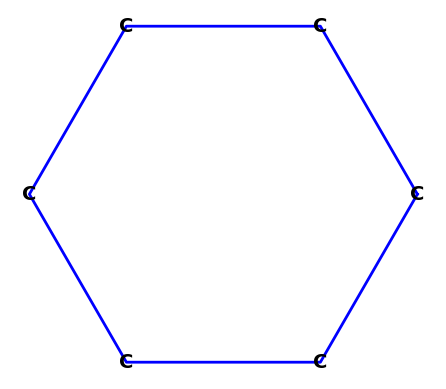
\includegraphics[width=0.5\textwidth]{benzene} \\[0.5cm]
                \Large Point Group: \textbf{D6h}
            \end{center}\newpage\section*{p orbitals}
Symmetry behavior of the p-orbitals:
$$\Gamma_{red} = \,6 E\;\oplus{}\,-2 C'2\;\oplus{}\,-6 \sigma h\;\oplus{}\,2 \sigma v\;$$
$$\Gamma_{irred} = \,1 B2g\;\oplus{}\,1 E1g\;\oplus{}\,1 A2u\;\oplus{}\,1 E2u\;$$


\begin{itemize}
\item SALC of B2g: \quad $\frac{\sqrt{6} p_{1}}{6} - \frac{\sqrt{6} p_{2}}{6} + \frac{\sqrt{6} p_{3}}{6} - \frac{\sqrt{6} p_{4}}{6} + \frac{\sqrt{6} p_{5}}{6} - \frac{\sqrt{6} p_{6}}{6}$
\item SALC of E1g: \quad $\frac{\sqrt{3} p_{1}}{3} + \frac{\sqrt{3} p_{2}}{6} - \frac{\sqrt{3} p_{3}}{6} - \frac{\sqrt{3} p_{4}}{3} - \frac{\sqrt{3} p_{5}}{6} + \frac{\sqrt{3} p_{6}}{6}$
\item SALC of E1g: \quad $\frac{p_{2}}{2} + \frac{p_{3}}{2} - \frac{p_{5}}{2} - \frac{p_{6}}{2}$
\item SALC of A2u: \quad $\frac{\sqrt{6} p_{1}}{6} + \frac{\sqrt{6} p_{2}}{6} + \frac{\sqrt{6} p_{3}}{6} + \frac{\sqrt{6} p_{4}}{6} + \frac{\sqrt{6} p_{5}}{6} + \frac{\sqrt{6} p_{6}}{6}$
\item SALC of E2u: \quad $\frac{\sqrt{3} p_{1}}{3} - \frac{\sqrt{3} p_{2}}{6} - \frac{\sqrt{3} p_{3}}{6} + \frac{\sqrt{3} p_{4}}{3} - \frac{\sqrt{3} p_{5}}{6} - \frac{\sqrt{3} p_{6}}{6}$
\item SALC of E2u: \quad $\frac{p_{2}}{2} - \frac{p_{3}}{2} + \frac{p_{5}}{2} - \frac{p_{6}}{2}$
\end{itemize}
Put together these SALCs form the following Hamilton matrices:
     $$ H_{B2g}= \left[\begin{bmatrix}\alpha - 2 \beta\end{bmatrix}\right]$$ 
     $$ H_{E1g}= \left[\begin{bmatrix}\alpha + \beta & 0\\0 & \alpha + \beta\end{bmatrix}\right]$$ 
     $$ H_{A2u}= \left[\begin{bmatrix}\alpha + 2 \beta\end{bmatrix}\right]$$ 
     $$ H_{E2u}= \left[\begin{bmatrix}\alpha - \beta & 0\\0 & \alpha - \beta\end{bmatrix}\right]$$ 


Solving Hückels secular equations, that follow from these H, leads to:
\begin{itemize}
\item orbital of A2u with energy = $\alpha + 2 \beta$
\item orbital of E1g with energy = $\alpha + \beta$
\item orbital of E1g with energy = $\alpha + \beta$
\item orbital of E2u with energy = $\alpha - \beta$
\item orbital of E2u with energy = $\alpha - \beta$
\item orbital of B2g with energy = $\alpha - 2 \beta$
\end{itemize}



\newpage \section*{s orbitals}
Symmetry behavior of the s-orbitals:
$$\Gamma_{red} = \,6 E\;\oplus{}\,2 C'2\;\oplus{}\,6 \sigma h\;\oplus{}\,2 \sigma v\;$$
$$\Gamma_{irred} = \,1 A1g\;\oplus{}\,1 E2g\;\oplus{}\,1 B1u\;\oplus{}\,1 E1u\;$$


\begin{itemize}
\item SALC of A1g: \quad $\frac{\sqrt{6} s_{1}}{6} + \frac{\sqrt{6} s_{2}}{6} + \frac{\sqrt{6} s_{3}}{6} + \frac{\sqrt{6} s_{4}}{6} + \frac{\sqrt{6} s_{5}}{6} + \frac{\sqrt{6} s_{6}}{6}$
\item SALC of E2g: \quad $\frac{\sqrt{3} s_{1}}{3} - \frac{\sqrt{3} s_{2}}{6} - \frac{\sqrt{3} s_{3}}{6} + \frac{\sqrt{3} s_{4}}{3} - \frac{\sqrt{3} s_{5}}{6} - \frac{\sqrt{3} s_{6}}{6}$
\item SALC of E2g: \quad $\frac{s_{2}}{2} - \frac{s_{3}}{2} + \frac{s_{5}}{2} - \frac{s_{6}}{2}$
\item SALC of B1u: \quad $\frac{\sqrt{6} s_{1}}{6} - \frac{\sqrt{6} s_{2}}{6} + \frac{\sqrt{6} s_{3}}{6} - \frac{\sqrt{6} s_{4}}{6} + \frac{\sqrt{6} s_{5}}{6} - \frac{\sqrt{6} s_{6}}{6}$
\item SALC of E1u: \quad $\frac{\sqrt{3} s_{1}}{3} + \frac{\sqrt{3} s_{2}}{6} - \frac{\sqrt{3} s_{3}}{6} - \frac{\sqrt{3} s_{4}}{3} - \frac{\sqrt{3} s_{5}}{6} + \frac{\sqrt{3} s_{6}}{6}$
\item SALC of E1u: \quad $\frac{s_{2}}{2} + \frac{s_{3}}{2} - \frac{s_{5}}{2} - \frac{s_{6}}{2}$
\end{itemize}
Put together these SALCs form the following Hamilton matrices:
     $$ H_{A1g}= \left[\begin{bmatrix}\alpha_{s} + 2 \beta_{s}\end{bmatrix}\right]$$ 
     $$ H_{E2g}= \left[\begin{bmatrix}\alpha_{s} - \beta_{s} & 0\\0 & \alpha_{s} - \beta_{s}\end{bmatrix}\right]$$ 
     $$ H_{B1u}= \left[\begin{bmatrix}\alpha_{s} - 2 \beta_{s}\end{bmatrix}\right]$$ 
     $$ H_{E1u}= \left[\begin{bmatrix}\alpha_{s} + \beta_{s} & 0\\0 & \alpha_{s} + \beta_{s}\end{bmatrix}\right]$$ 


Solving Hückels secular equations, that follow from these H, leads to:
\begin{itemize}
\item orbital of A1g with energy = $\alpha_{s} + 2 \beta_{s}$
\item orbital of E1u with energy = $\alpha_{s} + \beta_{s}$
\item orbital of E1u with energy = $\alpha_{s} + \beta_{s}$
\item orbital of E2g with energy = $\alpha_{s} - \beta_{s}$
\item orbital of E2g with energy = $\alpha_{s} - \beta_{s}$
\item orbital of B1u with energy = $\alpha_{s} - 2 \beta_{s}$
\end{itemize}



\newpage \section*{Transitions from p orbitals into s orbitals}\subsection*{State with Occupation [2, 2, 2, 0, 0, 0] (0 unpaired electrons, mult 1.0)}
        \noindent\textbf{Transition from $\phi_{2}$ into $\phi_{s_{2}}$:}
        \begin{itemize}
            \item $- [2, 2, 2, 0, 0, 0], (0, 0, 0, 0, 0, 0) \rightarrow (2, 1, 2, 0, 0, 0), (0, 1, 0, 0, 0, 0)$
        
            \item $\phi_{2}:$ linear combination = $\frac{\sqrt{3} p_{1}}{3} + \frac{\sqrt{3} p_{2}}{6} - \frac{\sqrt{3} p_{3}}{6} - \frac{\sqrt{3} p_{4}}{3} - \frac{\sqrt{3} p_{5}}{6} + \frac{\sqrt{3} p_{6}}{6}$, \
            energy = $\alpha + \beta$
            
            \item $\xi_{2}:$ linear combination = $\frac{\sqrt{3} s_{1}}{3} + \frac{\sqrt{3} s_{2}}{6} - \frac{\sqrt{3} s_{3}}{6} - \frac{\sqrt{3} s_{4}}{3} - \frac{\sqrt{3} s_{5}}{6} + \frac{\sqrt{3} s_{6}}{6}$, \
            energy = $\alpha_{s} + \beta_{s}$
            
            \item $\Delta$ Energy: $- \alpha + \alpha_{s} - \beta + \beta_{s}$
            \item Energy of State before Excitation: $6 \alpha + 8 \beta$
            \item Energy of State after Excitation: $5 \alpha + \alpha_{s} + 7 \beta + \beta_{s}$
            \item Energy between Average Energies of $\phi$-/$\xi$-orbitals: \
            $- \alpha + \alpha_{s}$
        
            \item dipole transition moment: $\delta$
        
        \end{itemize}
        

        \noindent\textbf{Transition from $\phi_{3}$ into $\phi_{s_{3}}$:}
        \begin{itemize}
            \item $- [2, 2, 2, 0, 0, 0], (0, 0, 0, 0, 0, 0) \rightarrow (2, 2, 1, 0, 0, 0), (0, 0, 1, 0, 0, 0)$
        
            \item $\phi_{3}:$ linear combination = $\frac{p_{2}}{2} + \frac{p_{3}}{2} - \frac{p_{5}}{2} - \frac{p_{6}}{2}$, \
            energy = $\alpha + \beta$
            
            \item $\xi_{3}:$ linear combination = $\frac{s_{2}}{2} + \frac{s_{3}}{2} - \frac{s_{5}}{2} - \frac{s_{6}}{2}$, \
            energy = $\alpha_{s} + \beta_{s}$
            
            \item $\Delta$ Energy: $- \alpha + \alpha_{s} - \beta + \beta_{s}$
            \item Energy of State before Excitation: $6 \alpha + 8 \beta$
            \item Energy of State after Excitation: $5 \alpha + \alpha_{s} + 7 \beta + \beta_{s}$
            \item Energy between Average Energies of $\phi$-/$\xi$-orbitals: \
            $- \alpha + \alpha_{s}$
        
            \item dipole transition moment: $\delta$
        
        \end{itemize}
        
\subsection*{State with Occupation (2, 1, 1, 1, 1, 0) (4 unpaired electrons, mult 5.0)}
        \noindent\textbf{Transition from $\phi_{2}$ into $\phi_{s_{2}}$:}
        \begin{itemize}
            \item $- (2, 1, 1, 1, 1, 0), (0, 0, 0, 0, 0, 0) \rightarrow (2, 0, 1, 1, 1, 0), (0, 1, 0, 0, 0, 0)$
        
            \item $\phi_{2}:$ linear combination = $\frac{\sqrt{3} p_{1}}{3} + \frac{\sqrt{3} p_{2}}{6} - \frac{\sqrt{3} p_{3}}{6} - \frac{\sqrt{3} p_{4}}{3} - \frac{\sqrt{3} p_{5}}{6} + \frac{\sqrt{3} p_{6}}{6}$, \
            energy = $\alpha + \beta$
            
            \item $\xi_{2}:$ linear combination = $\frac{\sqrt{3} s_{1}}{3} + \frac{\sqrt{3} s_{2}}{6} - \frac{\sqrt{3} s_{3}}{6} - \frac{\sqrt{3} s_{4}}{3} - \frac{\sqrt{3} s_{5}}{6} + \frac{\sqrt{3} s_{6}}{6}$, \
            energy = $\alpha_{s} + \beta_{s}$
            
            \item $\Delta$ Energy: $- \alpha + \alpha_{s} - \beta + \beta_{s}$
            \item Energy of State before Excitation: $6 \alpha + 4 \beta$
            \item Energy of State after Excitation: $5 \alpha + \alpha_{s} + 3 \beta + \beta_{s}$
            \item Energy between Average Energies of $\phi$-/$\xi$-orbitals: \
            $- \alpha + \alpha_{s}$
        
            \item dipole transition moment: $\delta$
        
        \end{itemize}
        

        \noindent\textbf{Transition from $\phi_{3}$ into $\phi_{s_{3}}$:}
        \begin{itemize}
            \item $- (2, 1, 1, 1, 1, 0), (0, 0, 0, 0, 0, 0) \rightarrow (2, 1, 0, 1, 1, 0), (0, 0, 1, 0, 0, 0)$
        
            \item $\phi_{3}:$ linear combination = $\frac{p_{2}}{2} + \frac{p_{3}}{2} - \frac{p_{5}}{2} - \frac{p_{6}}{2}$, \
            energy = $\alpha + \beta$
            
            \item $\xi_{3}:$ linear combination = $\frac{s_{2}}{2} + \frac{s_{3}}{2} - \frac{s_{5}}{2} - \frac{s_{6}}{2}$, \
            energy = $\alpha_{s} + \beta_{s}$
            
            \item $\Delta$ Energy: $- \alpha + \alpha_{s} - \beta + \beta_{s}$
            \item Energy of State before Excitation: $6 \alpha + 4 \beta$
            \item Energy of State after Excitation: $5 \alpha + \alpha_{s} + 3 \beta + \beta_{s}$
            \item Energy between Average Energies of $\phi$-/$\xi$-orbitals: \
            $- \alpha + \alpha_{s}$
        
            \item dipole transition moment: $\delta$
        
        \end{itemize}
        

        \noindent\textbf{Transition from $\phi_{4}$ into $\phi_{s_{4}}$:}
        \begin{itemize}
            \item $- (2, 1, 1, 1, 1, 0), (0, 0, 0, 0, 0, 0) \rightarrow (2, 1, 1, 0, 1, 0), (0, 0, 0, 1, 0, 0)$
        
            \item $\phi_{4}:$ linear combination = $\frac{\sqrt{3} p_{1}}{3} - \frac{\sqrt{3} p_{2}}{6} - \frac{\sqrt{3} p_{3}}{6} + \frac{\sqrt{3} p_{4}}{3} - \frac{\sqrt{3} p_{5}}{6} - \frac{\sqrt{3} p_{6}}{6}$, \
            energy = $\alpha - \beta$
            
            \item $\xi_{4}:$ linear combination = $\frac{\sqrt{3} s_{1}}{3} - \frac{\sqrt{3} s_{2}}{6} - \frac{\sqrt{3} s_{3}}{6} + \frac{\sqrt{3} s_{4}}{3} - \frac{\sqrt{3} s_{5}}{6} - \frac{\sqrt{3} s_{6}}{6}$, \
            energy = $\alpha_{s} - \beta_{s}$
            
            \item $\Delta$ Energy: $- \alpha + \alpha_{s} + \beta - \beta_{s}$
            \item Energy of State before Excitation: $6 \alpha + 4 \beta$
            \item Energy of State after Excitation: $5 \alpha + \alpha_{s} + 5 \beta - \beta_{s}$
            \item Energy between Average Energies of $\phi$-/$\xi$-orbitals: \
            $- \alpha + \alpha_{s}$
        
            \item dipole transition moment: $\delta$
        
        \end{itemize}
        

        \noindent\textbf{Transition from $\phi_{5}$ into $\phi_{s_{5}}$:}
        \begin{itemize}
            \item $- (2, 1, 1, 1, 1, 0), (0, 0, 0, 0, 0, 0) \rightarrow (2, 1, 1, 1, 0, 0), (0, 0, 0, 0, 1, 0)$
        
            \item $\phi_{5}:$ linear combination = $\frac{p_{2}}{2} - \frac{p_{3}}{2} + \frac{p_{5}}{2} - \frac{p_{6}}{2}$, \
            energy = $\alpha - \beta$
            
            \item $\xi_{5}:$ linear combination = $\frac{s_{2}}{2} - \frac{s_{3}}{2} + \frac{s_{5}}{2} - \frac{s_{6}}{2}$, \
            energy = $\alpha_{s} - \beta_{s}$
            
            \item $\Delta$ Energy: $- \alpha + \alpha_{s} + \beta - \beta_{s}$
            \item Energy of State before Excitation: $6 \alpha + 4 \beta$
            \item Energy of State after Excitation: $5 \alpha + \alpha_{s} + 5 \beta - \beta_{s}$
            \item Energy between Average Energies of $\phi$-/$\xi$-orbitals: \
            $- \alpha + \alpha_{s}$
        
            \item dipole transition moment: $\delta$
        
        \end{itemize}
        
\subsection*{State with Occupation (2, 1, 2, 0, 1, 0) (2 unpaired electrons, mult 3.0)}
        \noindent\textbf{Transition from $\phi_{2}$ into $\phi_{s_{2}}$:}
        \begin{itemize}
            \item $- (2, 1, 2, 0, 1, 0), (0, 0, 0, 0, 0, 0) \rightarrow (2, 0, 2, 0, 1, 0), (0, 1, 0, 0, 0, 0)$
        
            \item $\phi_{2}:$ linear combination = $\frac{\sqrt{3} p_{1}}{3} + \frac{\sqrt{3} p_{2}}{6} - \frac{\sqrt{3} p_{3}}{6} - \frac{\sqrt{3} p_{4}}{3} - \frac{\sqrt{3} p_{5}}{6} + \frac{\sqrt{3} p_{6}}{6}$, \
            energy = $\alpha + \beta$
            
            \item $\xi_{2}:$ linear combination = $\frac{\sqrt{3} s_{1}}{3} + \frac{\sqrt{3} s_{2}}{6} - \frac{\sqrt{3} s_{3}}{6} - \frac{\sqrt{3} s_{4}}{3} - \frac{\sqrt{3} s_{5}}{6} + \frac{\sqrt{3} s_{6}}{6}$, \
            energy = $\alpha_{s} + \beta_{s}$
            
            \item $\Delta$ Energy: $- \alpha + \alpha_{s} - \beta + \beta_{s}$
            \item Energy of State before Excitation: $6 \alpha + 6 \beta$
            \item Energy of State after Excitation: $5 \alpha + \alpha_{s} + 5 \beta + \beta_{s}$
            \item Energy between Average Energies of $\phi$-/$\xi$-orbitals: \
            $- \alpha + \alpha_{s}$
        
            \item dipole transition moment: $\delta$
        
        \end{itemize}
        

        \noindent\textbf{Transition from $\phi_{3}$ into $\phi_{s_{3}}$:}
        \begin{itemize}
            \item $- (2, 1, 2, 0, 1, 0), (0, 0, 0, 0, 0, 0) \rightarrow (2, 1, 1, 0, 1, 0), (0, 0, 1, 0, 0, 0)$
        
            \item $\phi_{3}:$ linear combination = $\frac{p_{2}}{2} + \frac{p_{3}}{2} - \frac{p_{5}}{2} - \frac{p_{6}}{2}$, \
            energy = $\alpha + \beta$
            
            \item $\xi_{3}:$ linear combination = $\frac{s_{2}}{2} + \frac{s_{3}}{2} - \frac{s_{5}}{2} - \frac{s_{6}}{2}$, \
            energy = $\alpha_{s} + \beta_{s}$
            
            \item $\Delta$ Energy: $- \alpha + \alpha_{s} - \beta + \beta_{s}$
            \item Energy of State before Excitation: $6 \alpha + 6 \beta$
            \item Energy of State after Excitation: $5 \alpha + \alpha_{s} + 5 \beta + \beta_{s}$
            \item Energy between Average Energies of $\phi$-/$\xi$-orbitals: \
            $- \alpha + \alpha_{s}$
        
            \item dipole transition moment: $\delta$
        
        \end{itemize}
        

        \noindent\textbf{Transition from $\phi_{5}$ into $\phi_{s_{5}}$:}
        \begin{itemize}
            \item $- (2, 1, 2, 0, 1, 0), (0, 0, 0, 0, 0, 0) \rightarrow (2, 1, 2, 0, 0, 0), (0, 0, 0, 0, 1, 0)$
        
            \item $\phi_{5}:$ linear combination = $\frac{p_{2}}{2} - \frac{p_{3}}{2} + \frac{p_{5}}{2} - \frac{p_{6}}{2}$, \
            energy = $\alpha - \beta$
            
            \item $\xi_{5}:$ linear combination = $\frac{s_{2}}{2} - \frac{s_{3}}{2} + \frac{s_{5}}{2} - \frac{s_{6}}{2}$, \
            energy = $\alpha_{s} - \beta_{s}$
            
            \item $\Delta$ Energy: $- \alpha + \alpha_{s} + \beta - \beta_{s}$
            \item Energy of State before Excitation: $6 \alpha + 6 \beta$
            \item Energy of State after Excitation: $5 \alpha + \alpha_{s} + 7 \beta - \beta_{s}$
            \item Energy between Average Energies of $\phi$-/$\xi$-orbitals: \
            $- \alpha + \alpha_{s}$
        
            \item dipole transition moment: $\delta$
        
        \end{itemize}
        
\subsection*{State with Occupation (2, 1, 2, 1, 0, 0) (2 unpaired electrons, mult 3.0)}
        \noindent\textbf{Transition from $\phi_{2}$ into $\phi_{s_{2}}$:}
        \begin{itemize}
            \item $- (2, 1, 2, 1, 0, 0), (0, 0, 0, 0, 0, 0) \rightarrow (2, 0, 2, 1, 0, 0), (0, 1, 0, 0, 0, 0)$
        
            \item $\phi_{2}:$ linear combination = $\frac{\sqrt{3} p_{1}}{3} + \frac{\sqrt{3} p_{2}}{6} - \frac{\sqrt{3} p_{3}}{6} - \frac{\sqrt{3} p_{4}}{3} - \frac{\sqrt{3} p_{5}}{6} + \frac{\sqrt{3} p_{6}}{6}$, \
            energy = $\alpha + \beta$
            
            \item $\xi_{2}:$ linear combination = $\frac{\sqrt{3} s_{1}}{3} + \frac{\sqrt{3} s_{2}}{6} - \frac{\sqrt{3} s_{3}}{6} - \frac{\sqrt{3} s_{4}}{3} - \frac{\sqrt{3} s_{5}}{6} + \frac{\sqrt{3} s_{6}}{6}$, \
            energy = $\alpha_{s} + \beta_{s}$
            
            \item $\Delta$ Energy: $- \alpha + \alpha_{s} - \beta + \beta_{s}$
            \item Energy of State before Excitation: $6 \alpha + 6 \beta$
            \item Energy of State after Excitation: $5 \alpha + \alpha_{s} + 5 \beta + \beta_{s}$
            \item Energy between Average Energies of $\phi$-/$\xi$-orbitals: \
            $- \alpha + \alpha_{s}$
        
            \item dipole transition moment: $\delta$
        
        \end{itemize}
        

        \noindent\textbf{Transition from $\phi_{3}$ into $\phi_{s_{3}}$:}
        \begin{itemize}
            \item $- (2, 1, 2, 1, 0, 0), (0, 0, 0, 0, 0, 0) \rightarrow (2, 1, 1, 1, 0, 0), (0, 0, 1, 0, 0, 0)$
        
            \item $\phi_{3}:$ linear combination = $\frac{p_{2}}{2} + \frac{p_{3}}{2} - \frac{p_{5}}{2} - \frac{p_{6}}{2}$, \
            energy = $\alpha + \beta$
            
            \item $\xi_{3}:$ linear combination = $\frac{s_{2}}{2} + \frac{s_{3}}{2} - \frac{s_{5}}{2} - \frac{s_{6}}{2}$, \
            energy = $\alpha_{s} + \beta_{s}$
            
            \item $\Delta$ Energy: $- \alpha + \alpha_{s} - \beta + \beta_{s}$
            \item Energy of State before Excitation: $6 \alpha + 6 \beta$
            \item Energy of State after Excitation: $5 \alpha + \alpha_{s} + 5 \beta + \beta_{s}$
            \item Energy between Average Energies of $\phi$-/$\xi$-orbitals: \
            $- \alpha + \alpha_{s}$
        
            \item dipole transition moment: $\delta$
        
        \end{itemize}
        

        \noindent\textbf{Transition from $\phi_{4}$ into $\phi_{s_{4}}$:}
        \begin{itemize}
            \item $- (2, 1, 2, 1, 0, 0), (0, 0, 0, 0, 0, 0) \rightarrow (2, 1, 2, 0, 0, 0), (0, 0, 0, 1, 0, 0)$
        
            \item $\phi_{4}:$ linear combination = $\frac{\sqrt{3} p_{1}}{3} - \frac{\sqrt{3} p_{2}}{6} - \frac{\sqrt{3} p_{3}}{6} + \frac{\sqrt{3} p_{4}}{3} - \frac{\sqrt{3} p_{5}}{6} - \frac{\sqrt{3} p_{6}}{6}$, \
            energy = $\alpha - \beta$
            
            \item $\xi_{4}:$ linear combination = $\frac{\sqrt{3} s_{1}}{3} - \frac{\sqrt{3} s_{2}}{6} - \frac{\sqrt{3} s_{3}}{6} + \frac{\sqrt{3} s_{4}}{3} - \frac{\sqrt{3} s_{5}}{6} - \frac{\sqrt{3} s_{6}}{6}$, \
            energy = $\alpha_{s} - \beta_{s}$
            
            \item $\Delta$ Energy: $- \alpha + \alpha_{s} + \beta - \beta_{s}$
            \item Energy of State before Excitation: $6 \alpha + 6 \beta$
            \item Energy of State after Excitation: $5 \alpha + \alpha_{s} + 7 \beta - \beta_{s}$
            \item Energy between Average Energies of $\phi$-/$\xi$-orbitals: \
            $- \alpha + \alpha_{s}$
        
            \item dipole transition moment: $\delta$
        
        \end{itemize}
        
\subsection*{State with Occupation (2, 2, 1, 0, 1, 0) (2 unpaired electrons, mult 3.0)}
        \noindent\textbf{Transition from $\phi_{2}$ into $\phi_{s_{2}}$:}
        \begin{itemize}
            \item $- (2, 2, 1, 0, 1, 0), (0, 0, 0, 0, 0, 0) \rightarrow (2, 1, 1, 0, 1, 0), (0, 1, 0, 0, 0, 0)$
        
            \item $\phi_{2}:$ linear combination = $\frac{\sqrt{3} p_{1}}{3} + \frac{\sqrt{3} p_{2}}{6} - \frac{\sqrt{3} p_{3}}{6} - \frac{\sqrt{3} p_{4}}{3} - \frac{\sqrt{3} p_{5}}{6} + \frac{\sqrt{3} p_{6}}{6}$, \
            energy = $\alpha + \beta$
            
            \item $\xi_{2}:$ linear combination = $\frac{\sqrt{3} s_{1}}{3} + \frac{\sqrt{3} s_{2}}{6} - \frac{\sqrt{3} s_{3}}{6} - \frac{\sqrt{3} s_{4}}{3} - \frac{\sqrt{3} s_{5}}{6} + \frac{\sqrt{3} s_{6}}{6}$, \
            energy = $\alpha_{s} + \beta_{s}$
            
            \item $\Delta$ Energy: $- \alpha + \alpha_{s} - \beta + \beta_{s}$
            \item Energy of State before Excitation: $6 \alpha + 6 \beta$
            \item Energy of State after Excitation: $5 \alpha + \alpha_{s} + 5 \beta + \beta_{s}$
            \item Energy between Average Energies of $\phi$-/$\xi$-orbitals: \
            $- \alpha + \alpha_{s}$
        
            \item dipole transition moment: $\delta$
        
        \end{itemize}
        

        \noindent\textbf{Transition from $\phi_{3}$ into $\phi_{s_{3}}$:}
        \begin{itemize}
            \item $- (2, 2, 1, 0, 1, 0), (0, 0, 0, 0, 0, 0) \rightarrow (2, 2, 0, 0, 1, 0), (0, 0, 1, 0, 0, 0)$
        
            \item $\phi_{3}:$ linear combination = $\frac{p_{2}}{2} + \frac{p_{3}}{2} - \frac{p_{5}}{2} - \frac{p_{6}}{2}$, \
            energy = $\alpha + \beta$
            
            \item $\xi_{3}:$ linear combination = $\frac{s_{2}}{2} + \frac{s_{3}}{2} - \frac{s_{5}}{2} - \frac{s_{6}}{2}$, \
            energy = $\alpha_{s} + \beta_{s}$
            
            \item $\Delta$ Energy: $- \alpha + \alpha_{s} - \beta + \beta_{s}$
            \item Energy of State before Excitation: $6 \alpha + 6 \beta$
            \item Energy of State after Excitation: $5 \alpha + \alpha_{s} + 5 \beta + \beta_{s}$
            \item Energy between Average Energies of $\phi$-/$\xi$-orbitals: \
            $- \alpha + \alpha_{s}$
        
            \item dipole transition moment: $\delta$
        
        \end{itemize}
        

        \noindent\textbf{Transition from $\phi_{5}$ into $\phi_{s_{5}}$:}
        \begin{itemize}
            \item $- (2, 2, 1, 0, 1, 0), (0, 0, 0, 0, 0, 0) \rightarrow (2, 2, 1, 0, 0, 0), (0, 0, 0, 0, 1, 0)$
        
            \item $\phi_{5}:$ linear combination = $\frac{p_{2}}{2} - \frac{p_{3}}{2} + \frac{p_{5}}{2} - \frac{p_{6}}{2}$, \
            energy = $\alpha - \beta$
            
            \item $\xi_{5}:$ linear combination = $\frac{s_{2}}{2} - \frac{s_{3}}{2} + \frac{s_{5}}{2} - \frac{s_{6}}{2}$, \
            energy = $\alpha_{s} - \beta_{s}$
            
            \item $\Delta$ Energy: $- \alpha + \alpha_{s} + \beta - \beta_{s}$
            \item Energy of State before Excitation: $6 \alpha + 6 \beta$
            \item Energy of State after Excitation: $5 \alpha + \alpha_{s} + 7 \beta - \beta_{s}$
            \item Energy between Average Energies of $\phi$-/$\xi$-orbitals: \
            $- \alpha + \alpha_{s}$
        
            \item dipole transition moment: $\delta$
        
        \end{itemize}
        
\subsection*{State with Occupation (2, 2, 1, 1, 0, 0) (2 unpaired electrons, mult 3.0)}
        \noindent\textbf{Transition from $\phi_{2}$ into $\phi_{s_{2}}$:}
        \begin{itemize}
            \item $- (2, 2, 1, 1, 0, 0), (0, 0, 0, 0, 0, 0) \rightarrow (2, 1, 1, 1, 0, 0), (0, 1, 0, 0, 0, 0)$
        
            \item $\phi_{2}:$ linear combination = $\frac{\sqrt{3} p_{1}}{3} + \frac{\sqrt{3} p_{2}}{6} - \frac{\sqrt{3} p_{3}}{6} - \frac{\sqrt{3} p_{4}}{3} - \frac{\sqrt{3} p_{5}}{6} + \frac{\sqrt{3} p_{6}}{6}$, \
            energy = $\alpha + \beta$
            
            \item $\xi_{2}:$ linear combination = $\frac{\sqrt{3} s_{1}}{3} + \frac{\sqrt{3} s_{2}}{6} - \frac{\sqrt{3} s_{3}}{6} - \frac{\sqrt{3} s_{4}}{3} - \frac{\sqrt{3} s_{5}}{6} + \frac{\sqrt{3} s_{6}}{6}$, \
            energy = $\alpha_{s} + \beta_{s}$
            
            \item $\Delta$ Energy: $- \alpha + \alpha_{s} - \beta + \beta_{s}$
            \item Energy of State before Excitation: $6 \alpha + 6 \beta$
            \item Energy of State after Excitation: $5 \alpha + \alpha_{s} + 5 \beta + \beta_{s}$
            \item Energy between Average Energies of $\phi$-/$\xi$-orbitals: \
            $- \alpha + \alpha_{s}$
        
            \item dipole transition moment: $\delta$
        
        \end{itemize}
        

        \noindent\textbf{Transition from $\phi_{3}$ into $\phi_{s_{3}}$:}
        \begin{itemize}
            \item $- (2, 2, 1, 1, 0, 0), (0, 0, 0, 0, 0, 0) \rightarrow (2, 2, 0, 1, 0, 0), (0, 0, 1, 0, 0, 0)$
        
            \item $\phi_{3}:$ linear combination = $\frac{p_{2}}{2} + \frac{p_{3}}{2} - \frac{p_{5}}{2} - \frac{p_{6}}{2}$, \
            energy = $\alpha + \beta$
            
            \item $\xi_{3}:$ linear combination = $\frac{s_{2}}{2} + \frac{s_{3}}{2} - \frac{s_{5}}{2} - \frac{s_{6}}{2}$, \
            energy = $\alpha_{s} + \beta_{s}$
            
            \item $\Delta$ Energy: $- \alpha + \alpha_{s} - \beta + \beta_{s}$
            \item Energy of State before Excitation: $6 \alpha + 6 \beta$
            \item Energy of State after Excitation: $5 \alpha + \alpha_{s} + 5 \beta + \beta_{s}$
            \item Energy between Average Energies of $\phi$-/$\xi$-orbitals: \
            $- \alpha + \alpha_{s}$
        
            \item dipole transition moment: $\delta$
        
        \end{itemize}
        

        \noindent\textbf{Transition from $\phi_{4}$ into $\phi_{s_{4}}$:}
        \begin{itemize}
            \item $- (2, 2, 1, 1, 0, 0), (0, 0, 0, 0, 0, 0) \rightarrow (2, 2, 1, 0, 0, 0), (0, 0, 0, 1, 0, 0)$
        
            \item $\phi_{4}:$ linear combination = $\frac{\sqrt{3} p_{1}}{3} - \frac{\sqrt{3} p_{2}}{6} - \frac{\sqrt{3} p_{3}}{6} + \frac{\sqrt{3} p_{4}}{3} - \frac{\sqrt{3} p_{5}}{6} - \frac{\sqrt{3} p_{6}}{6}$, \
            energy = $\alpha - \beta$
            
            \item $\xi_{4}:$ linear combination = $\frac{\sqrt{3} s_{1}}{3} - \frac{\sqrt{3} s_{2}}{6} - \frac{\sqrt{3} s_{3}}{6} + \frac{\sqrt{3} s_{4}}{3} - \frac{\sqrt{3} s_{5}}{6} - \frac{\sqrt{3} s_{6}}{6}$, \
            energy = $\alpha_{s} - \beta_{s}$
            
            \item $\Delta$ Energy: $- \alpha + \alpha_{s} + \beta - \beta_{s}$
            \item Energy of State before Excitation: $6 \alpha + 6 \beta$
            \item Energy of State after Excitation: $5 \alpha + \alpha_{s} + 7 \beta - \beta_{s}$
            \item Energy between Average Energies of $\phi$-/$\xi$-orbitals: \
            $- \alpha + \alpha_{s}$
        
            \item dipole transition moment: $\delta$
        
        \end{itemize}
        
\newpage \section*{Dispersion energies following from the transitions}

\begin{enumerate}
 \item State: A = [2, 2, 2, 0, 0, 0] $\leftrightarrow$ B = (2, 1, 1, 1, 1, 0) 
$$E_{dispersion} =\frac{16 \delta^{4} \left(- 2 \alpha + 2 \alpha_{s} - \beta + \beta_{s}\right)}{r^{6} \left(\alpha - \alpha_{s}\right) \left(\alpha - \alpha_{s} + \beta - \beta_{s}\right)}$$
 \item State: A = (2, 1, 1, 1, 1, 0) $\leftrightarrow$ B = [2, 2, 2, 0, 0, 0] 
$$E_{dispersion} =\frac{16 \delta^{4} \left(- 2 \alpha + 2 \alpha_{s} - \beta + \beta_{s}\right)}{r^{6} \left(\alpha - \alpha_{s}\right) \left(\alpha - \alpha_{s} + \beta - \beta_{s}\right)}$$
 \item State: A = (2, 1, 2, 0, 1, 0) $\leftrightarrow$ B = (2, 1, 2, 0, 1, 0) 
$$E_{dispersion} =\frac{2 \delta^{4} \left(- 9 \left(\alpha - \alpha_{s}\right) \left(\alpha - \alpha_{s} - \beta + \beta_{s}\right) - \left(\alpha - \alpha_{s}\right) \left(\alpha - \alpha_{s} + \beta - \beta_{s}\right) - 6 \left(\alpha - \alpha_{s} - \beta + \beta_{s}\right) \left(\alpha - \alpha_{s} + \beta - \beta_{s}\right)\right)}{r^{6} \left(\alpha - \alpha_{s}\right) \left(\alpha - \alpha_{s} - \beta + \beta_{s}\right) \left(\alpha - \alpha_{s} + \beta - \beta_{s}\right)}$$
 \item State: A = (2, 1, 2, 0, 1, 0) $\leftrightarrow$ B = (2, 1, 2, 1, 0, 0) 
$$E_{dispersion} =\frac{2 \delta^{4} \left(- 9 \left(\alpha - \alpha_{s}\right) \left(\alpha - \alpha_{s} - \beta + \beta_{s}\right) - \left(\alpha - \alpha_{s}\right) \left(\alpha - \alpha_{s} + \beta - \beta_{s}\right) - 6 \left(\alpha - \alpha_{s} - \beta + \beta_{s}\right) \left(\alpha - \alpha_{s} + \beta - \beta_{s}\right)\right)}{r^{6} \left(\alpha - \alpha_{s}\right) \left(\alpha - \alpha_{s} - \beta + \beta_{s}\right) \left(\alpha - \alpha_{s} + \beta - \beta_{s}\right)}$$
 \item State: A = (2, 1, 2, 0, 1, 0) $\leftrightarrow$ B = (2, 2, 1, 0, 1, 0) 
$$E_{dispersion} =\frac{2 \delta^{4} \left(- 9 \left(\alpha - \alpha_{s}\right) \left(\alpha - \alpha_{s} - \beta + \beta_{s}\right) - \left(\alpha - \alpha_{s}\right) \left(\alpha - \alpha_{s} + \beta - \beta_{s}\right) - 6 \left(\alpha - \alpha_{s} - \beta + \beta_{s}\right) \left(\alpha - \alpha_{s} + \beta - \beta_{s}\right)\right)}{r^{6} \left(\alpha - \alpha_{s}\right) \left(\alpha - \alpha_{s} - \beta + \beta_{s}\right) \left(\alpha - \alpha_{s} + \beta - \beta_{s}\right)}$$
 \item State: A = (2, 1, 2, 0, 1, 0) $\leftrightarrow$ B = (2, 2, 1, 1, 0, 0) 
$$E_{dispersion} =\frac{2 \delta^{4} \left(- 9 \left(\alpha - \alpha_{s}\right) \left(\alpha - \alpha_{s} - \beta + \beta_{s}\right) - \left(\alpha - \alpha_{s}\right) \left(\alpha - \alpha_{s} + \beta - \beta_{s}\right) - 6 \left(\alpha - \alpha_{s} - \beta + \beta_{s}\right) \left(\alpha - \alpha_{s} + \beta - \beta_{s}\right)\right)}{r^{6} \left(\alpha - \alpha_{s}\right) \left(\alpha - \alpha_{s} - \beta + \beta_{s}\right) \left(\alpha - \alpha_{s} + \beta - \beta_{s}\right)}$$
 \item State: A = (2, 1, 2, 1, 0, 0) $\leftrightarrow$ B = (2, 1, 2, 0, 1, 0) 
$$E_{dispersion} =\frac{2 \delta^{4} \left(- 9 \left(\alpha - \alpha_{s}\right) \left(\alpha - \alpha_{s} - \beta + \beta_{s}\right) - \left(\alpha - \alpha_{s}\right) \left(\alpha - \alpha_{s} + \beta - \beta_{s}\right) - 6 \left(\alpha - \alpha_{s} - \beta + \beta_{s}\right) \left(\alpha - \alpha_{s} + \beta - \beta_{s}\right)\right)}{r^{6} \left(\alpha - \alpha_{s}\right) \left(\alpha - \alpha_{s} - \beta + \beta_{s}\right) \left(\alpha - \alpha_{s} + \beta - \beta_{s}\right)}$$
 \item State: A = (2, 1, 2, 1, 0, 0) $\leftrightarrow$ B = (2, 1, 2, 1, 0, 0) 
$$E_{dispersion} =\frac{2 \delta^{4} \left(- 9 \left(\alpha - \alpha_{s}\right) \left(\alpha - \alpha_{s} - \beta + \beta_{s}\right) - \left(\alpha - \alpha_{s}\right) \left(\alpha - \alpha_{s} + \beta - \beta_{s}\right) - 6 \left(\alpha - \alpha_{s} - \beta + \beta_{s}\right) \left(\alpha - \alpha_{s} + \beta - \beta_{s}\right)\right)}{r^{6} \left(\alpha - \alpha_{s}\right) \left(\alpha - \alpha_{s} - \beta + \beta_{s}\right) \left(\alpha - \alpha_{s} + \beta - \beta_{s}\right)}$$
 \item State: A = (2, 1, 2, 1, 0, 0) $\leftrightarrow$ B = (2, 2, 1, 0, 1, 0) 
$$E_{dispersion} =\frac{2 \delta^{4} \left(- 9 \left(\alpha - \alpha_{s}\right) \left(\alpha - \alpha_{s} - \beta + \beta_{s}\right) - \left(\alpha - \alpha_{s}\right) \left(\alpha - \alpha_{s} + \beta - \beta_{s}\right) - 6 \left(\alpha - \alpha_{s} - \beta + \beta_{s}\right) \left(\alpha - \alpha_{s} + \beta - \beta_{s}\right)\right)}{r^{6} \left(\alpha - \alpha_{s}\right) \left(\alpha - \alpha_{s} - \beta + \beta_{s}\right) \left(\alpha - \alpha_{s} + \beta - \beta_{s}\right)}$$
 \item State: A = (2, 1, 2, 1, 0, 0) $\leftrightarrow$ B = (2, 2, 1, 1, 0, 0) 
$$E_{dispersion} =\frac{2 \delta^{4} \left(- 9 \left(\alpha - \alpha_{s}\right) \left(\alpha - \alpha_{s} - \beta + \beta_{s}\right) - \left(\alpha - \alpha_{s}\right) \left(\alpha - \alpha_{s} + \beta - \beta_{s}\right) - 6 \left(\alpha - \alpha_{s} - \beta + \beta_{s}\right) \left(\alpha - \alpha_{s} + \beta - \beta_{s}\right)\right)}{r^{6} \left(\alpha - \alpha_{s}\right) \left(\alpha - \alpha_{s} - \beta + \beta_{s}\right) \left(\alpha - \alpha_{s} + \beta - \beta_{s}\right)}$$
 \item State: A = (2, 2, 1, 0, 1, 0) $\leftrightarrow$ B = (2, 1, 2, 0, 1, 0) 
$$E_{dispersion} =\frac{2 \delta^{4} \left(- 9 \left(\alpha - \alpha_{s}\right) \left(\alpha - \alpha_{s} - \beta + \beta_{s}\right) - \left(\alpha - \alpha_{s}\right) \left(\alpha - \alpha_{s} + \beta - \beta_{s}\right) - 6 \left(\alpha - \alpha_{s} - \beta + \beta_{s}\right) \left(\alpha - \alpha_{s} + \beta - \beta_{s}\right)\right)}{r^{6} \left(\alpha - \alpha_{s}\right) \left(\alpha - \alpha_{s} - \beta + \beta_{s}\right) \left(\alpha - \alpha_{s} + \beta - \beta_{s}\right)}$$
 \item State: A = (2, 2, 1, 0, 1, 0) $\leftrightarrow$ B = (2, 1, 2, 1, 0, 0) 
$$E_{dispersion} =\frac{2 \delta^{4} \left(- 9 \left(\alpha - \alpha_{s}\right) \left(\alpha - \alpha_{s} - \beta + \beta_{s}\right) - \left(\alpha - \alpha_{s}\right) \left(\alpha - \alpha_{s} + \beta - \beta_{s}\right) - 6 \left(\alpha - \alpha_{s} - \beta + \beta_{s}\right) \left(\alpha - \alpha_{s} + \beta - \beta_{s}\right)\right)}{r^{6} \left(\alpha - \alpha_{s}\right) \left(\alpha - \alpha_{s} - \beta + \beta_{s}\right) \left(\alpha - \alpha_{s} + \beta - \beta_{s}\right)}$$
 \item State: A = (2, 2, 1, 0, 1, 0) $\leftrightarrow$ B = (2, 2, 1, 0, 1, 0) 
$$E_{dispersion} =\frac{2 \delta^{4} \left(- 9 \left(\alpha - \alpha_{s}\right) \left(\alpha - \alpha_{s} - \beta + \beta_{s}\right) - \left(\alpha - \alpha_{s}\right) \left(\alpha - \alpha_{s} + \beta - \beta_{s}\right) - 6 \left(\alpha - \alpha_{s} - \beta + \beta_{s}\right) \left(\alpha - \alpha_{s} + \beta - \beta_{s}\right)\right)}{r^{6} \left(\alpha - \alpha_{s}\right) \left(\alpha - \alpha_{s} - \beta + \beta_{s}\right) \left(\alpha - \alpha_{s} + \beta - \beta_{s}\right)}$$
 \item State: A = (2, 2, 1, 0, 1, 0) $\leftrightarrow$ B = (2, 2, 1, 1, 0, 0) 
$$E_{dispersion} =\frac{2 \delta^{4} \left(- 9 \left(\alpha - \alpha_{s}\right) \left(\alpha - \alpha_{s} - \beta + \beta_{s}\right) - \left(\alpha - \alpha_{s}\right) \left(\alpha - \alpha_{s} + \beta - \beta_{s}\right) - 6 \left(\alpha - \alpha_{s} - \beta + \beta_{s}\right) \left(\alpha - \alpha_{s} + \beta - \beta_{s}\right)\right)}{r^{6} \left(\alpha - \alpha_{s}\right) \left(\alpha - \alpha_{s} - \beta + \beta_{s}\right) \left(\alpha - \alpha_{s} + \beta - \beta_{s}\right)}$$
 \item State: A = (2, 2, 1, 1, 0, 0) $\leftrightarrow$ B = (2, 1, 2, 0, 1, 0) 
$$E_{dispersion} =\frac{2 \delta^{4} \left(- 9 \left(\alpha - \alpha_{s}\right) \left(\alpha - \alpha_{s} - \beta + \beta_{s}\right) - \left(\alpha - \alpha_{s}\right) \left(\alpha - \alpha_{s} + \beta - \beta_{s}\right) - 6 \left(\alpha - \alpha_{s} - \beta + \beta_{s}\right) \left(\alpha - \alpha_{s} + \beta - \beta_{s}\right)\right)}{r^{6} \left(\alpha - \alpha_{s}\right) \left(\alpha - \alpha_{s} - \beta + \beta_{s}\right) \left(\alpha - \alpha_{s} + \beta - \beta_{s}\right)}$$
 \item State: A = (2, 2, 1, 1, 0, 0) $\leftrightarrow$ B = (2, 1, 2, 1, 0, 0) 
$$E_{dispersion} =\frac{2 \delta^{4} \left(- 9 \left(\alpha - \alpha_{s}\right) \left(\alpha - \alpha_{s} - \beta + \beta_{s}\right) - \left(\alpha - \alpha_{s}\right) \left(\alpha - \alpha_{s} + \beta - \beta_{s}\right) - 6 \left(\alpha - \alpha_{s} - \beta + \beta_{s}\right) \left(\alpha - \alpha_{s} + \beta - \beta_{s}\right)\right)}{r^{6} \left(\alpha - \alpha_{s}\right) \left(\alpha - \alpha_{s} - \beta + \beta_{s}\right) \left(\alpha - \alpha_{s} + \beta - \beta_{s}\right)}$$
 \item State: A = (2, 2, 1, 1, 0, 0) $\leftrightarrow$ B = (2, 2, 1, 0, 1, 0) 
$$E_{dispersion} =\frac{2 \delta^{4} \left(- 9 \left(\alpha - \alpha_{s}\right) \left(\alpha - \alpha_{s} - \beta + \beta_{s}\right) - \left(\alpha - \alpha_{s}\right) \left(\alpha - \alpha_{s} + \beta - \beta_{s}\right) - 6 \left(\alpha - \alpha_{s} - \beta + \beta_{s}\right) \left(\alpha - \alpha_{s} + \beta - \beta_{s}\right)\right)}{r^{6} \left(\alpha - \alpha_{s}\right) \left(\alpha - \alpha_{s} - \beta + \beta_{s}\right) \left(\alpha - \alpha_{s} + \beta - \beta_{s}\right)}$$
 \item State: A = (2, 2, 1, 1, 0, 0) $\leftrightarrow$ B = (2, 2, 1, 1, 0, 0) 
$$E_{dispersion} =\frac{2 \delta^{4} \left(- 9 \left(\alpha - \alpha_{s}\right) \left(\alpha - \alpha_{s} - \beta + \beta_{s}\right) - \left(\alpha - \alpha_{s}\right) \left(\alpha - \alpha_{s} + \beta - \beta_{s}\right) - 6 \left(\alpha - \alpha_{s} - \beta + \beta_{s}\right) \left(\alpha - \alpha_{s} + \beta - \beta_{s}\right)\right)}{r^{6} \left(\alpha - \alpha_{s}\right) \left(\alpha - \alpha_{s} - \beta + \beta_{s}\right) \left(\alpha - \alpha_{s} + \beta - \beta_{s}\right)}$$
\end{enumerate}
\textcolor{red}{Error in Calculations Dispersion can only concatenate list (not "str") to list}

\end{document}